%----------------------------------------------------------------------------------------
%	LMU BEAMER TEMPLATE -- modern edition
%	Compile with pdflatex (2 runs, plus bibtex for the references)
%----------------------------------------------------------------------------------------

\documentclass[aspectratio=169, 10pt]{beamer}

%----------------------------------------------------------------------------------------
%	PACKAGES
%----------------------------------------------------------------------------------------
\usepackage[english]{babel}
\usepackage[utf8]{inputenc}
\usepackage[T1]{fontenc}
\usepackage[default]{sourcesanspro}   % font type
\usepackage{amsmath,amssymb}
\usepackage{graphicx}
\usepackage{booktabs}
\usepackage{hyperref}
\usepackage{tikz}
\usepackage{textpos}                  % logo position
\usepackage{appendixnumberbeamer}  % keeps page numbers sane with backup slides
\usepackage{adjustbox}
\usepackage{caption}
\usepackage{listings}
\usepackage{xcolor}

%----------------------------------------------------------------------------------------
%	COLORS  (LMU green + calm neutrals)
%----------------------------------------------------------------------------------------
\definecolor{lmugreen}{RGB}{0, 136, 58}
\definecolor{lmudark}{RGB}{0, 84, 36}        % darker green for emphasis
\definecolor{lmulight}{RGB}{229, 243, 235}   % very light green tint (block backgrounds)
\usepackage{colortbl}   % for \rowcolor

\newcommand{\hcell}[1]{\textcolor{white}{\textbf{#1}}}  % header cell
\newcommand{\best}[1]{\textbf{\textcolor{lmudark}{#1}}} % best value in column
\definecolor{textgray}{RGB}{38, 42, 40}      % body text, softer than pure black
\definecolor{midgray}{RGB}{130, 136, 133}    % footer, captions
\definecolor{linegray}{RGB}{215, 219, 217}   % thin rules

\setbeamercolor{normal text}{fg=textgray, bg=white}
\setbeamercolor{structure}{fg=lmugreen}
\setbeamercolor{alerted text}{fg=lmudark}
\setbeamercolor{frametitle}{fg=lmugreen, bg=white}
\setbeamercolor{title}{fg=white}
\setbeamercolor{footline text}{fg=midgray}
\hypersetup{colorlinks=true, linkcolor=lmugreen, urlcolor=lmugreen, citecolor=lmugreen}

%----------------------------------------------------------------------------------------
%	THEME: flat, no gradients, no navigation clutter
%----------------------------------------------------------------------------------------
\usetheme{default}
\beamertemplatenavigationsymbolsempty
\setbeamertemplate{caption}[numbered]
\captionsetup{font=scriptsize, labelfont={scriptsize,color=lmugreen}, justification=centering}

% --- Top progress bar (thin, LMU green) ---------------------------------------------
\setbeamertemplate{headline}{%
	\begin{tikzpicture}[remember picture, overlay]
		\fill[linegray] (current page.north west) rectangle ([yshift=-0.12cm]current page.north east);
		\fill[lmugreen] (current page.north west) rectangle
			([xshift={\paperwidth*\insertframenumber/\inserttotalframenumber}, yshift=-0.12cm]current page.north west);
	\end{tikzpicture}%
}

% --- Frame title: left-aligned, bold, green, thin rule below -------------------------
\setbeamertemplate{frametitle}{%
	\vspace{0.55cm}
	\begin{beamercolorbox}[wd=0.72\paperwidth, ht=1.2ex, dp=0ex, left]{frametitle}
		\usebeamerfont{frametitle}\insertframetitle
		\ifx\insertframesubtitle\empty\else
			\\[-0.4ex]{\usebeamerfont{framesubtitle}\color{midgray}\insertframesubtitle}
		\fi
	\end{beamercolorbox}
	\vspace{-0.1cm}
	{\color{linegray}\rule{\textwidth}{0.4pt}}%
}
\setbeamerfont{frametitle}{size=\Large, series=\bfseries}
\setbeamerfont{framesubtitle}{size=\small, series=\normalfont}

% Logo top right on every content frame
\addtobeamertemplate{frametitle}{}{%
	\begin{textblock*}{3cm}(\dimexpr\paperwidth-4cm\relax,-0.75cm)
		\raggedleft
\includegraphics[height=0.8cm,keepaspectratio]{lmu_logo}
	\end{textblock*}}

% --- Footer: author | title | page ---------------------------------------------------
\setbeamertemplate{footline}{%
	\leavevmode%
	\hbox{%
		\begin{beamercolorbox}[wd=.33\paperwidth, ht=3ex, dp=1.5ex, left, leftskip=1em]{footline text}
			\usebeamerfont{footline}\insertshortauthor
		\end{beamercolorbox}%
		\begin{beamercolorbox}[wd=.34\paperwidth, ht=3ex, dp=1.5ex, center]{footline text}
			\usebeamerfont{footline}\insertsectionhead
		\end{beamercolorbox}%
		\begin{beamercolorbox}[wd=.33\paperwidth, ht=3ex, dp=1.5ex, right, rightskip=1em]{footline text}
			\usebeamerfont{footline}{\color{lmugreen}\bfseries\insertframenumber}\,/\,\inserttotalframenumber
		\end{beamercolorbox}%
	}%
	\vskip0.2cm
}
\setbeamerfont{footline}{size=\tiny}

% --- Lists: small green squares/dashes ----------------------------------------------
\setbeamertemplate{itemize items}[square]
\setbeamertemplate{itemize item}{\scriptsize\raise0.1ex\hbox{\donotcoloroutermaths$\blacksquare$}}
\setbeamertemplate{itemize subitem}{\tiny\raise0.2ex\hbox{\donotcoloroutermaths$\blacksquare$}}
\setbeamercolor{itemize item}{fg=lmugreen}
\setbeamercolor{itemize subitem}{fg=lmugreen!60!white}
\setbeamertemplate{enumerate items}[default]
\setbeamercolor{enumerate item}{fg=lmugreen}
\setlength{\leftmargini}{1.2em}

% --- Blocks: flat box with a green left bar -----------------------------------------
\setbeamertemplate{blocks}[default]
\setbeamercolor{block title}{fg=lmudark, bg=lmulight}
\setbeamercolor{block body}{fg=textgray, bg=lmulight!55!white}
\setbeamercolor{block title alerted}{fg=white, bg=lmudark}
\setbeamercolor{block body alerted}{fg=textgray, bg=lmulight!55!white}
\setbeamercolor{block title example}{fg=lmudark, bg=lmulight}
\setbeamercolor{block body example}{fg=textgray, bg=lmulight!55!white}
\setbeamerfont{block title}{size=\small, series=\bfseries}

% --- Section divider: big number, quiet layout --------------------------------------
\setbeamerfont{section title}{size=\Huge, series=\bfseries}
\AtBeginSection[]{%
	\begin{frame}[noframenumbering, plain]
		\begin{tikzpicture}[remember picture, overlay]
			\fill[lmugreen] (current page.south west) rectangle
				([xshift=0.9cm]current page.north west);
			\node[anchor=west, text=lmugreen, font=\fontsize{64}{64}\selectfont\bfseries]
				at ([xshift=2cm, yshift=0.6cm]current page.west) {\thesection};
			\node[anchor=west, text=textgray, font=\Huge\bfseries, align=left, text width=0.7\paperwidth]
				at ([xshift=2cm, yshift=-0.9cm]current page.west) {\insertsection};
		\end{tikzpicture}
	\end{frame}
}

% --- Code listings (R) --------------------------------------------------------------
\lstset{
	language=R,
	basicstyle=\scriptsize\ttfamily\color{textgray},
	commentstyle=\ttfamily\color{midgray},
	keywordstyle=\color{lmudark}\bfseries,
	stringstyle=\color{lmugreen},
	backgroundcolor=\color{lmulight!45!white},
	frame=l, rulecolor=\color{lmugreen}, framerule=2pt,
	xleftmargin=0.6em, framexleftmargin=0.6em,
	showspaces=false, showstringspaces=false, showtabs=false,
	tabsize=2, captionpos=b, breaklines=true,
}

% --- Outline (table of contents) ------------------------------------------------------
\setbeamercolor{section in toc}{fg=textgray}
\setbeamertemplate{section in toc}[sections numbered]
\setbeamercolor{section number projected}{bg=lmugreen, fg=white}
\setbeamercolor{item projected}{bg=lmugreen, fg=white}

%----------------------------------------------------------------------------------------
%	TITLE INFO
%----------------------------------------------------------------------------------------
\title[Reasoning Traces]{Reasoning models and reasoning traces}
\subtitle{What are they and how useful are they for
information extraction?}
\author[Regina Pichler, Eliana Tondar]{Regina Pichler, Eliana Tondar}
\institute[LMU]{Ludwig-Maximilians-Universit\"at M\"unchen \\
GIST / Master's seminar}
\date{\today}

\begin{document}

%----------------------------------------------------------------------------------------
%	TITLE PAGE (LMU background: title in the green block, details on the right)
%	Geometry of lmu-background.pdf (16:9, 16 x 9 cm): green block is ~6.5 cm wide.
%	Adjust the two lengths below if the text should sit differently.
%----------------------------------------------------------------------------------------
\newcommand{\greenblockwidth}{5.2cm}   % text width inside the green block
\newcommand{\rightblockx}{7.4cm}       % left edge of the text on the white side

{
\usebackgroundtemplate{
\includegraphics[width=\paperwidth]{lmu-background.pdf}}
\setbeamertemplate{headline}{}
\setbeamertemplate{footline}{}
\begin{frame}[plain, noframenumbering]
	\begin{tikzpicture}[remember picture, overlay]
		% Title + short rule inside the green block
		\node[anchor=north west, text width=\greenblockwidth, inner sep=0pt, align=left, text=white]
			at ([xshift=0.9cm, yshift=-2.2cm]current page.north west)
			{\hyphenpenalty=10000\exhyphenpenalty=10000\fontsize{20}{24}\selectfont\bfseries\inserttitle\par
			 \vspace{0.35cm}\rule{1.6cm}{1.5pt}};
		% Subtitle, author, institute, date on the white side
		\node[anchor=north west, text width=8cm, inner sep=0pt, align=left, text=textgray]
			at ([xshift=\rightblockx, yshift=-2.2cm]current page.north west)
			{{\color{lmugreen}\large\bfseries\insertsubtitle\par}
			 \vspace{0.7cm}
			 {\bfseries\insertauthor\par}
			 \vspace{0.25cm}
			 {\footnotesize\insertinstitute\par}
			 \vspace{0.35cm}
			 {\footnotesize\color{midgray}\insertdate\par}};
	\end{tikzpicture}
\end{frame}
}


\begin{frame}{Outline}
	\tableofcontents
\end{frame}

%========================================================================================
\section{Background}

\begin{frame}{Background}
\begin{itemize}
  \item \textbf{Task:} extract GHG / KPI values from sustainability reports
  \item \textbf{Pipeline:} ClimateXtract (retrieval $\rightarrow$ LLM $\rightarrow$ evaluation)
  \item \textbf{Models:} gpt-oss-120b, DeepSeek-V4-Flash
  \item \textbf{Variation:} reasoning effort (low / medium / high; high / max)
\end{itemize}
\vspace{0.6em}
\begin{block}{Central question}
What changes when reasoning effort changes -- in extraction quality,
and in the \textbf{visible reasoning traces}?
\end{block}
\end{frame}

\begin{frame}{Background -- What are reasoning traces?}
\begin{itemize}
  \item Reasoning models can emit visible intermediate text before the answer
  \item Higher effort allocates more reasoning budget -- not automatically better answers
  \item Visible traces are \textbf{generated text}, not a faithful record of internal computation
\end{itemize}
\end{frame}

\begin{frame}{Background -- Example traces}
\begin{columns}[T]

\begin{column}{0.36\textwidth}
\begin{block}{GPT-OSS low (46 words)}
\scriptsize\itshape
We need extract total emissions. Text says ``direct and indirect CO$_2$
emissions in fiscal 2021 were 1,053,000 tons.'' That's total Scope1+2? It's
direct and indirect = Scope1+2 combined, not separate. We need separate
values; not given. So none? No other absolute values. So output empty list.
\end{block}
\end{column}

\begin{column}{0.60\textwidth}
\begin{block}{GPT-OSS medium (193 words, shortened)}
\scriptsize\itshape
We need to extract absolute values for Scope 1, Scope 2 (market-based or
location-based), Scope 3 from the excerpt. Only values for whole company,
absolute numbers, not percentages. [\dots]
We have excerpt: ``The Fujifilm Group's direct and indirect CO$_2$ emissions in
fiscal 2021 were 1,053,000 tons.'' This seems to be total of direct (Scope 1) +
indirect (Scope 2?) [\dots] But we need separate values for each scope. [\dots]
Also later: ``our direct CO$_2$ emissions in fiscal 2021 were reduced by 3\% over
the fiscal 2019 level''. That's a relative change, not absolute. [\dots]
The instruction: ``Only extract value referring to Scope 1, Scope 2 or Scope 3
separately.'' [\dots] So we cannot extract combined total. [\dots]
Thus output empty \texttt{KPI\_Entries} array.
\end{block}
\end{column}

\end{columns}

\vspace{0.6em}
\begin{center}
$\rightarrow$ Same input, same answer -- medium checks more rules before concluding.
\end{center}
{\scriptsize Shortened}
\end{frame}
%========================================================================================
\section{Setup}

\begin{frame}{What is a reasoning trace?}
\begin{block}{Definition}
Visible reasoning text returned for one LLM call
(one retrieved page), separate from the final JSON answer.
\end{block}
\vspace{0.6em}
\begin{columns}[T]
\begin{column}{0.48\textwidth}
\textbf{Input}\\
excerpt + extraction prompt
\end{column}
\begin{column}{0.48\textwidth}
\textbf{Output}\\
1.\ reasoning trace\\
2.\ structured answer
\end{column}
\end{columns}
\end{frame}

\begin{frame}{Pipeline \& approach}
\begin{enumerate}
  \item Retrieve relevant pages from the PDF
  \item Query the LLM at a chosen reasoning effort
  \item Store trace, answer, tokens / cost
  \item Evaluate extractions against the gold standard
\end{enumerate}
\vspace{0.6em}
\footnotesize
Same corpus across runs; compare effort levels within and across models.
\end{frame}
%========================================================================================
\section{First Insights}


\begin{frame}{Where we are}
\begin{itemize}
  \item Completed runs:
    \begin{itemize}
        \item gpt-6-luna: reasoning none
        \item gpt-oss-120b: reasoning low, medium, high
        \item DeepSeek-V4-Flash-0731: reasoning none, high, max
    \end{itemize}
  \item Performance and cost can be compared
  \item Traces are available for analysis
\end{itemize}
\end{frame}



\begin{frame}{Model Performance}
\begin{columns}[c]
\begin{column}{0.60\textwidth}
\centering
\renewcommand{\arraystretch}{1.25}
\small
\begin{tabular}{l ccc}
\toprule
\rowcolor{lmugreen}
\hcell{Model} & \hcell{Precision} & \hcell{Recall} & \hcell{F1} \\
\midrule
Luna none      & 0.743 & 0.906 & 0.816 \\
\rowcolor{lmulight!60}
GPT-OSS low    & 0.758 & 0.762 & 0.760 \\
GPT-OSS medium & 0.759 & 0.845 & 0.800 \\
\rowcolor{lmulight!60}
GPT-OSS high   & 0.707 & 0.820 & 0.759 \\
DeepSeek none  & 0.719 & \best{0.913} & 0.805 \\
\rowcolor{lmulight!60}
DeepSeek high  & \best{0.846} & 0.869 & \best{0.857} \\
DeepSeek max   & 0.835 & 0.853 & 0.844 \\

\bottomrule
\end{tabular}
\end{column}

\begin{column}{0.36\textwidth}
\begin{block}{Definitions}
\footnotesize
\textbf{TP:} extracted value matches the gold value\\
\textbf{FP:} extracted value does not match the gold standard\\
\textbf{FN:} {gold standard exists, no value extracted}\\
\textbf{TN:} {no gold standard, no extracted value} \\[0.5em]
\textbf{Precision} $= \frac{TP}{TP+FP}$\\
\textbf{Recall} $= \frac{TP}{TP+FN}$\\
\textbf{F1}: harmonic mean of both
\end{block}
\end{column}
\end{columns}

\vspace{0.6em}
\centering
$\rightarrow$ Higher effort does not
consistently improve F1.
\end{frame}

\begin{frame}{F1 vs.\ Cost}
\centering
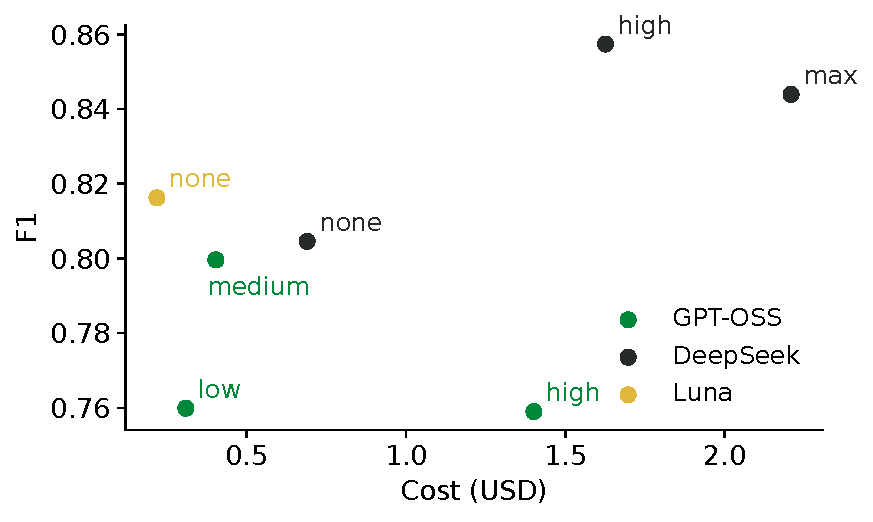
\includegraphics[height=0.75\textheight, keepaspectratio]{presentation/figures/cost_vs_f1.pdf}

\vspace{0.6em}
\centering
$\rightarrow$ Best trade-off: Luna none and DeepSeek high.
\end{frame}

\begin{frame}{Trace Statistics}
%lieber alles als mean vom call? -> Vergleichbarer
    \centering
\renewcommand{\arraystretch}{1.25}
\small
\begin{tabular}{l rr r rr}
\toprule
\rowcolor{lmugreen}
\hcell{Model}
  & \hcell{\shortstack[r]{Completion\\tokens (k)}}
  & \hcell{\shortstack[r]{Reasoning\\tokens (k)}}
  & \hcell{\shortstack[r]{Cost\\(USD)}}
  & \hcell{\shortstack[r]{Time/call (s)\\mean}}
  & \hcell{\shortstack[r]{sentences per\\reasoning trace (mean)}}\\
\midrule
Luna none      &    29 &    - & \best{0.22} &  2.4 & -  \\
\rowcolor{lmulight!60}
GPT-OSS low    &    87 &    44 & 0.31 &  1.6  & 4.5 \\
GPT-OSS medium &   244 &   201 & 0.40 &  2.5 & 16.3 \\
\rowcolor{lmulight!60}
GPT-OSS high   & 1{,}907 & 1{,}861 & 1.40 & 11.1 & 177.4 \\
DeepSeek none  &    46 &     - & 0.69 &  \best{1.2} & - \\
\rowcolor{lmulight!60}
DeepSeek high  &   820 &   790 & 1.63 & 12.4 & 59.3 \\
DeepSeek max   & 1{,}266 & 1{,}236 & 2.21 & 34.4 & 92.0 \\
\bottomrule
\end{tabular}
\end{frame}

\begin{frame}{Reasoning Tokens}
\centering
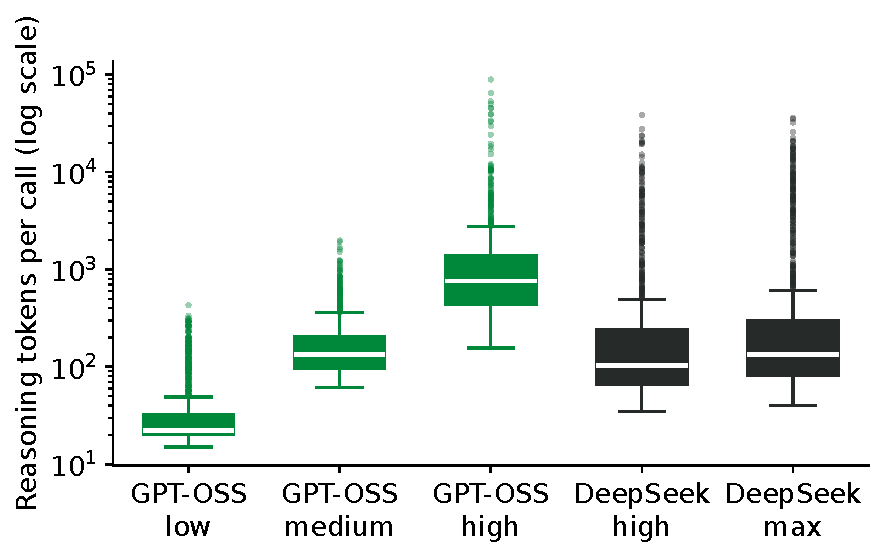
\includegraphics[height=0.75\textheight, keepaspectratio]{presentation/figures/reasoning_tokens_boxplot.pdf}
\end{frame}


\begin{frame}{Take-aways: First Insights}
    \begin{itemize}
        \item More reasoning changes cost and trace length, not necessarily quality
        \item Luna as none-reasoning better performance than every gpt-oss model with reasoning
    \end{itemize}
\end{frame}

%========================================================================================
\section{Analysis directions}

\begin{frame}{What we want to discuss today}
How should we analyse the traces?
\vspace{0.5em}
\begin{enumerate}
  \item \textbf{Topic modelling} -- what topics appear in the text?
  \item \textbf{Functions within the Trace} -- annotation scheme
  \item \textbf{LLM-as-a-judge} -- assign parts of trace to topics/functions
  \item \textbf{Error Analysis of Incorrect Traces}
  \item\textbf{Further Literature}
\end{enumerate}
\end{frame}

\begin{frame}{1.\ Topic modelling}
\begin{itemize}
  \item Goal: discover structure in reasoning sentences without a fixed codebook first
  \item Unit of analysis: sentences (not whole traces)
\end{itemize}
\vspace{0.4em}
\begin{center}
\small
\begin{tabular}{lll}
\toprule
Approach & Idea & Role \\
\midrule
Embeddings + BERTopic & semantic clusters & main exploratory method \\
LDA (counts) & classical bag-of-words & baseline \\
NMF (TF-IDF) & lexical factors & baseline \\
\bottomrule
\end{tabular}
\end{center}
\vspace{0.5em}
\begin{alertblock}{Open point}
Unsupervised clusters still need human labels -- and may not match evaluation criteria.
\end{alertblock}
\end{frame}

\begin{frame}{2.\ Functions within the Trace - ReasoningFlow }
\begin{columns}[c]
\begin{column}{0.42\textwidth}
\begin{itemize}
  \item Annotation scheme for complex reasoning traces
  \item \textbf{nodes} = semantic role, \\\textbf{edges} = relationship between nodes
  \item Goal: compare models and reasoning levels by the structure of traces
\end{itemize}
\end{column}

\begin{column}{0.56\textwidth}
\centering
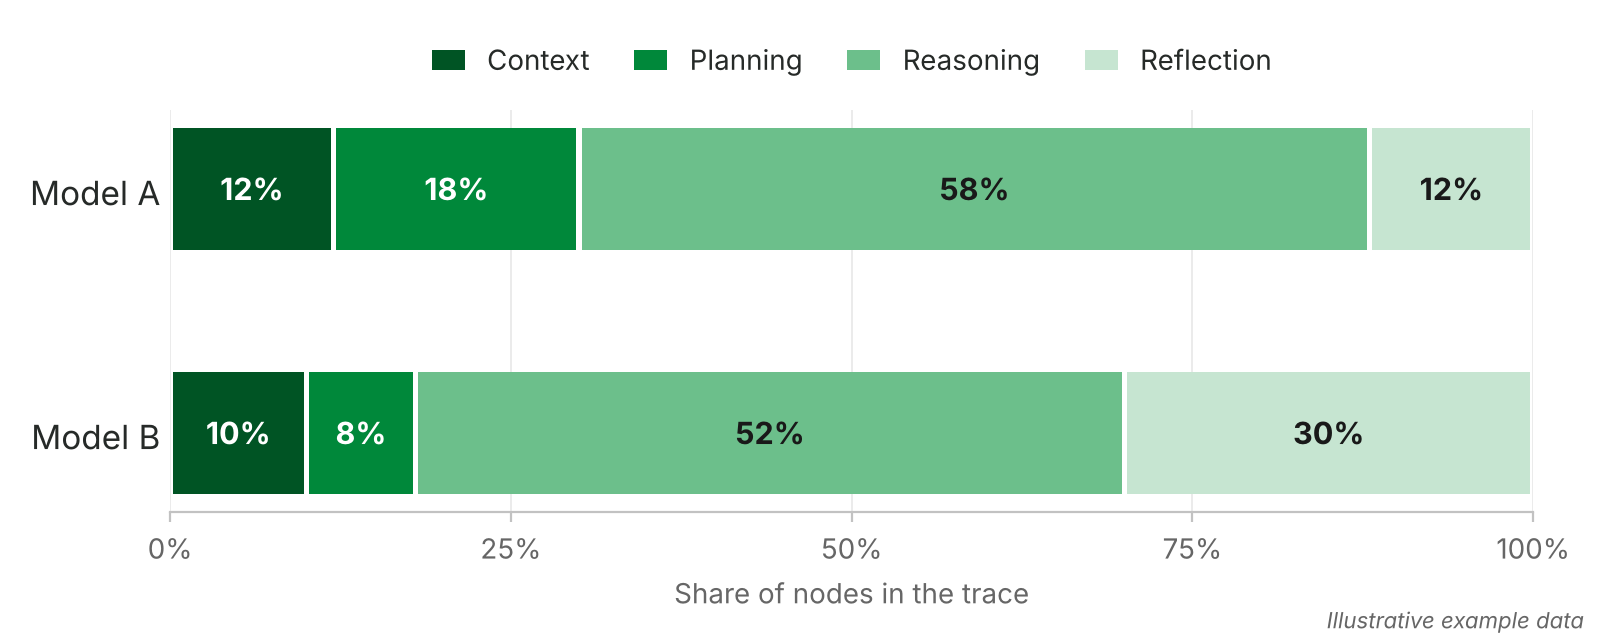
\includegraphics[width=\textwidth, keepaspectratio]{presentation/figures/node_types_stacked.png}
\end{column}
\end{columns}

\vspace{0.8em}
\begin{center}
$\rightarrow$ Does reasoning effort change the structure of a trace?
\end{center}

\end{frame}

\begin{frame}{ReasoningFlow -- Nodes and Edges}
\begin{columns}[T]

\begin{column}{0.52\textwidth}
\textbf{Nodes} {\footnotesize (what a step does)}\\[0.3em]
\renewcommand{\arraystretch}{1.1}
\footnotesize
\setlength{\tabcolsep}{4pt}
\begin{tabular}{p{0.26\columnwidth} p{0.68\columnwidth}}
\toprule
\rowcolor{lmugreen}
\hcell{Type} & \hcell{Meaning} \\
\midrule
Context     & Corresponds to provided text \\
\rowcolor{lmulight!60}
Planning    & Introduces content for following nodes \\
Fact        & Phrases containing external knowledge \\
\rowcolor{lmulight!60}
Reasoning   & Deductive / inductive / abductive inference \\
Restatement & Rephrases preceding text \\
\rowcolor{lmulight!60}
Assumption  & Proposition assumed for further reasoning \\
Example     & Example of a general concept / condition \\
\rowcolor{lmulight!60}
Reflection  & Confidence, feelings, impressions, doubt \\
Conclusion  & Contains the model's answer \\
\bottomrule
\end{tabular}
\end{column}

\begin{column}{0.44\textwidth}
\textbf{Edges} {\footnotesize (how steps relate)}\\[0.3em]
\renewcommand{\arraystretch}{1.1}
\footnotesize
\setlength{\tabcolsep}{4pt}
\begin{tabular}{p{0.28\columnwidth} p{0.66\columnwidth}}
\toprule
\rowcolor{lmugreen}
\hcell{Type} & \hcell{Meaning} \\
\midrule
Planning   & How plans arise, break down and follow each other \\
\rowcolor{lmulight!60}
Reasoning  & How content builds on earlier content \\
Evaluation & How the model judges earlier steps \\
\bottomrule
\end{tabular}

\end{column}

\end{columns}
\centering
\vspace{0.6em}
{\scriptsize Source: Lee et al.\ (2025), \textit{ReasoningFlow}}
\end{frame}

\newlength{\imgh}
\settoheight{\imgh}{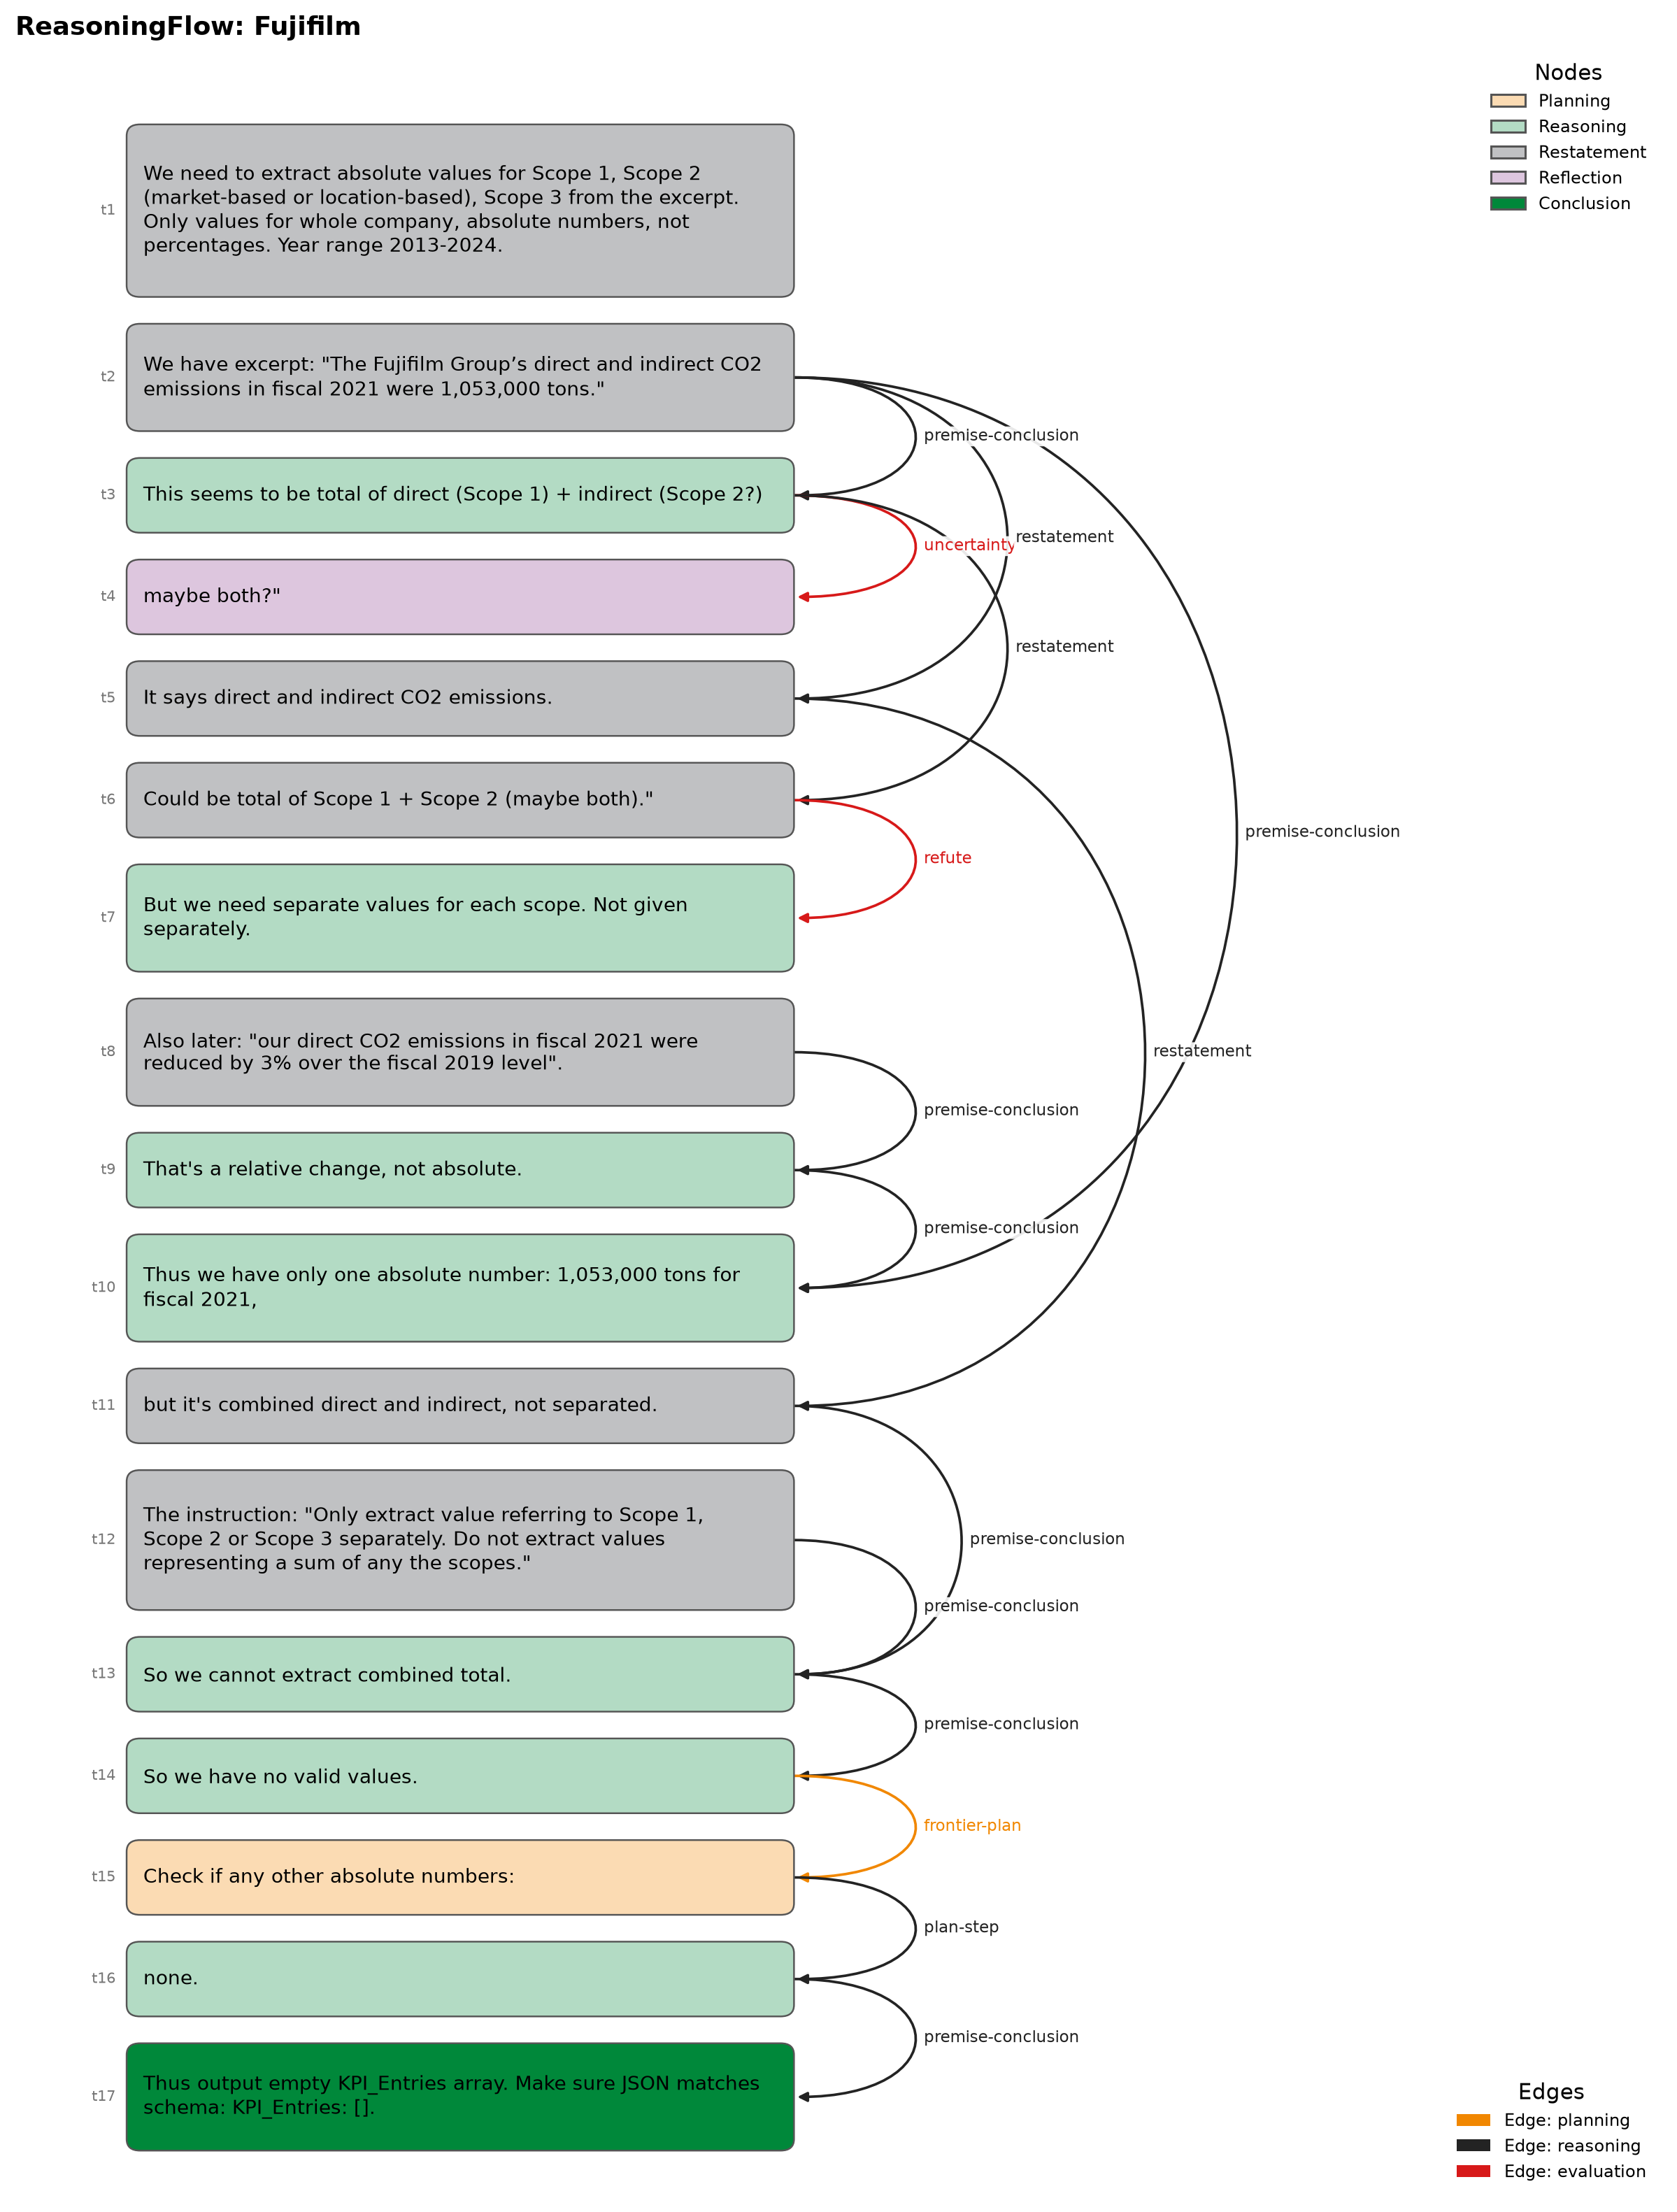
\includegraphics{presentation/figures/reasoningflow_fujifilm.png}}

\begin{frame}{ReasoningFlow -- Example}
\begin{columns}[T]

\begin{column}{0.49\textwidth}
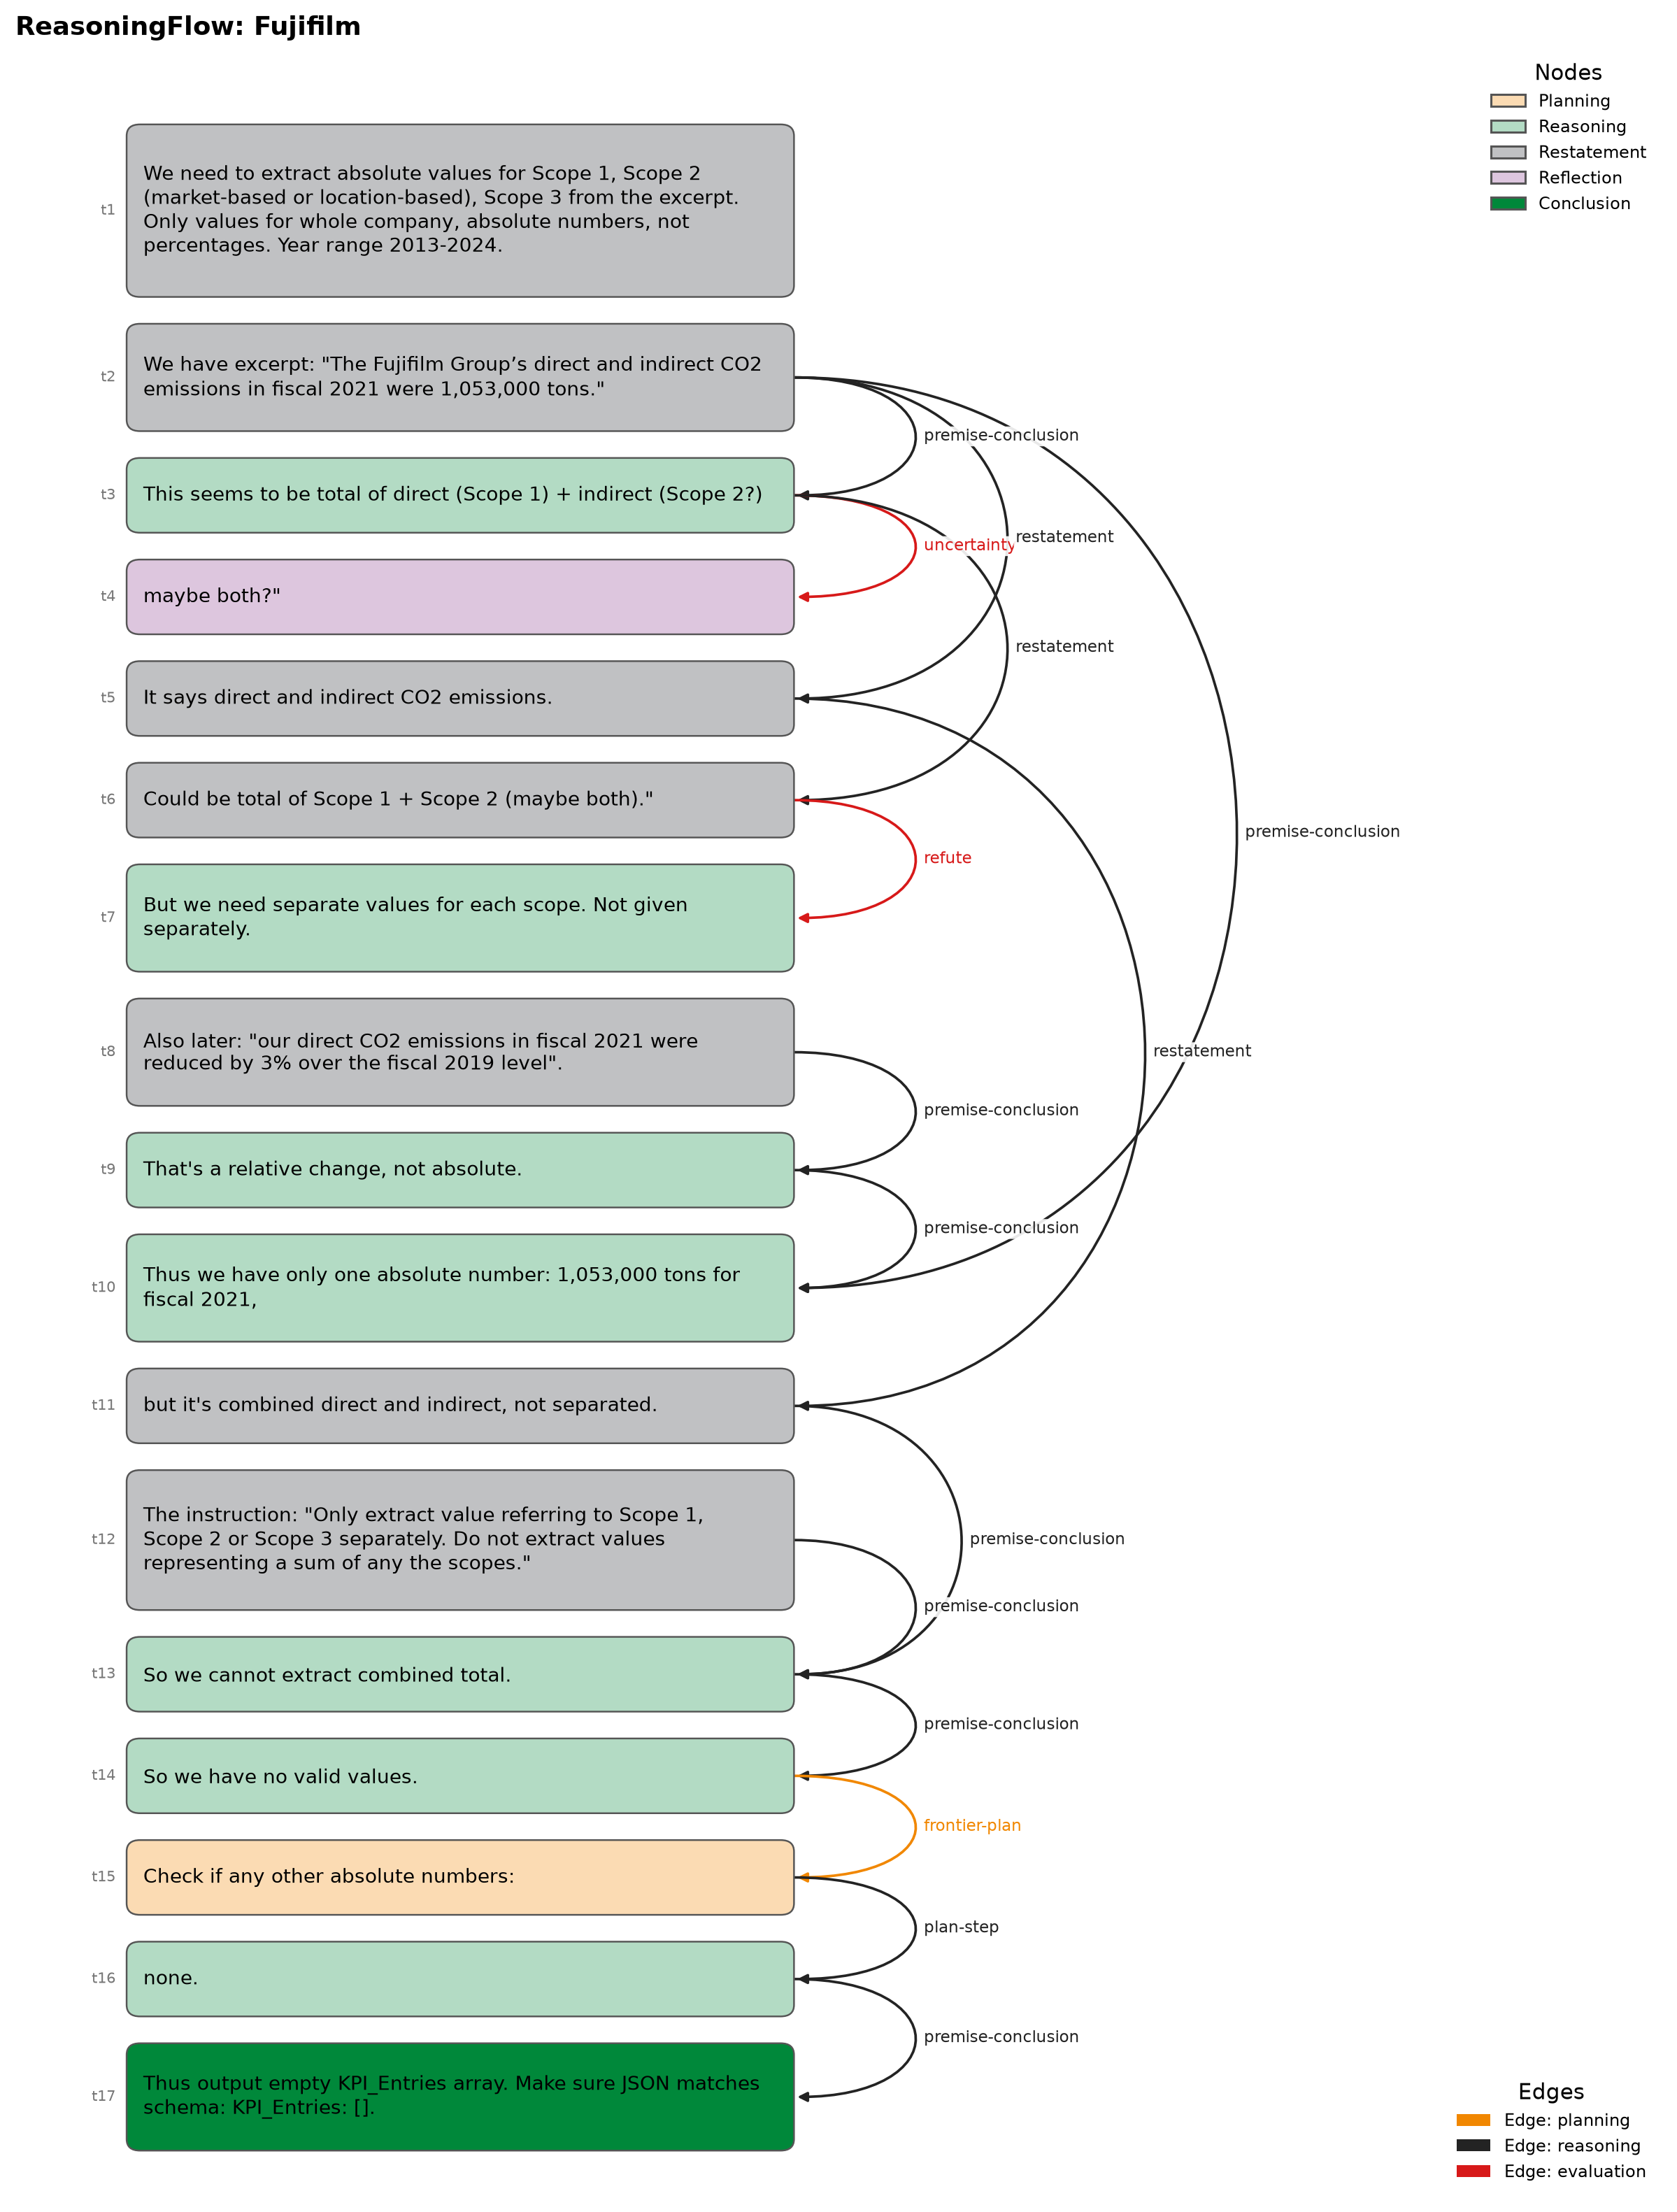
\includegraphics[trim=0pt {0.5\imgh} 0pt 0pt, clip, width=\columnwidth]{presentation/figures/reasoningflow_fujifilm.png}
\end{column}

\begin{column}{0.49\textwidth}
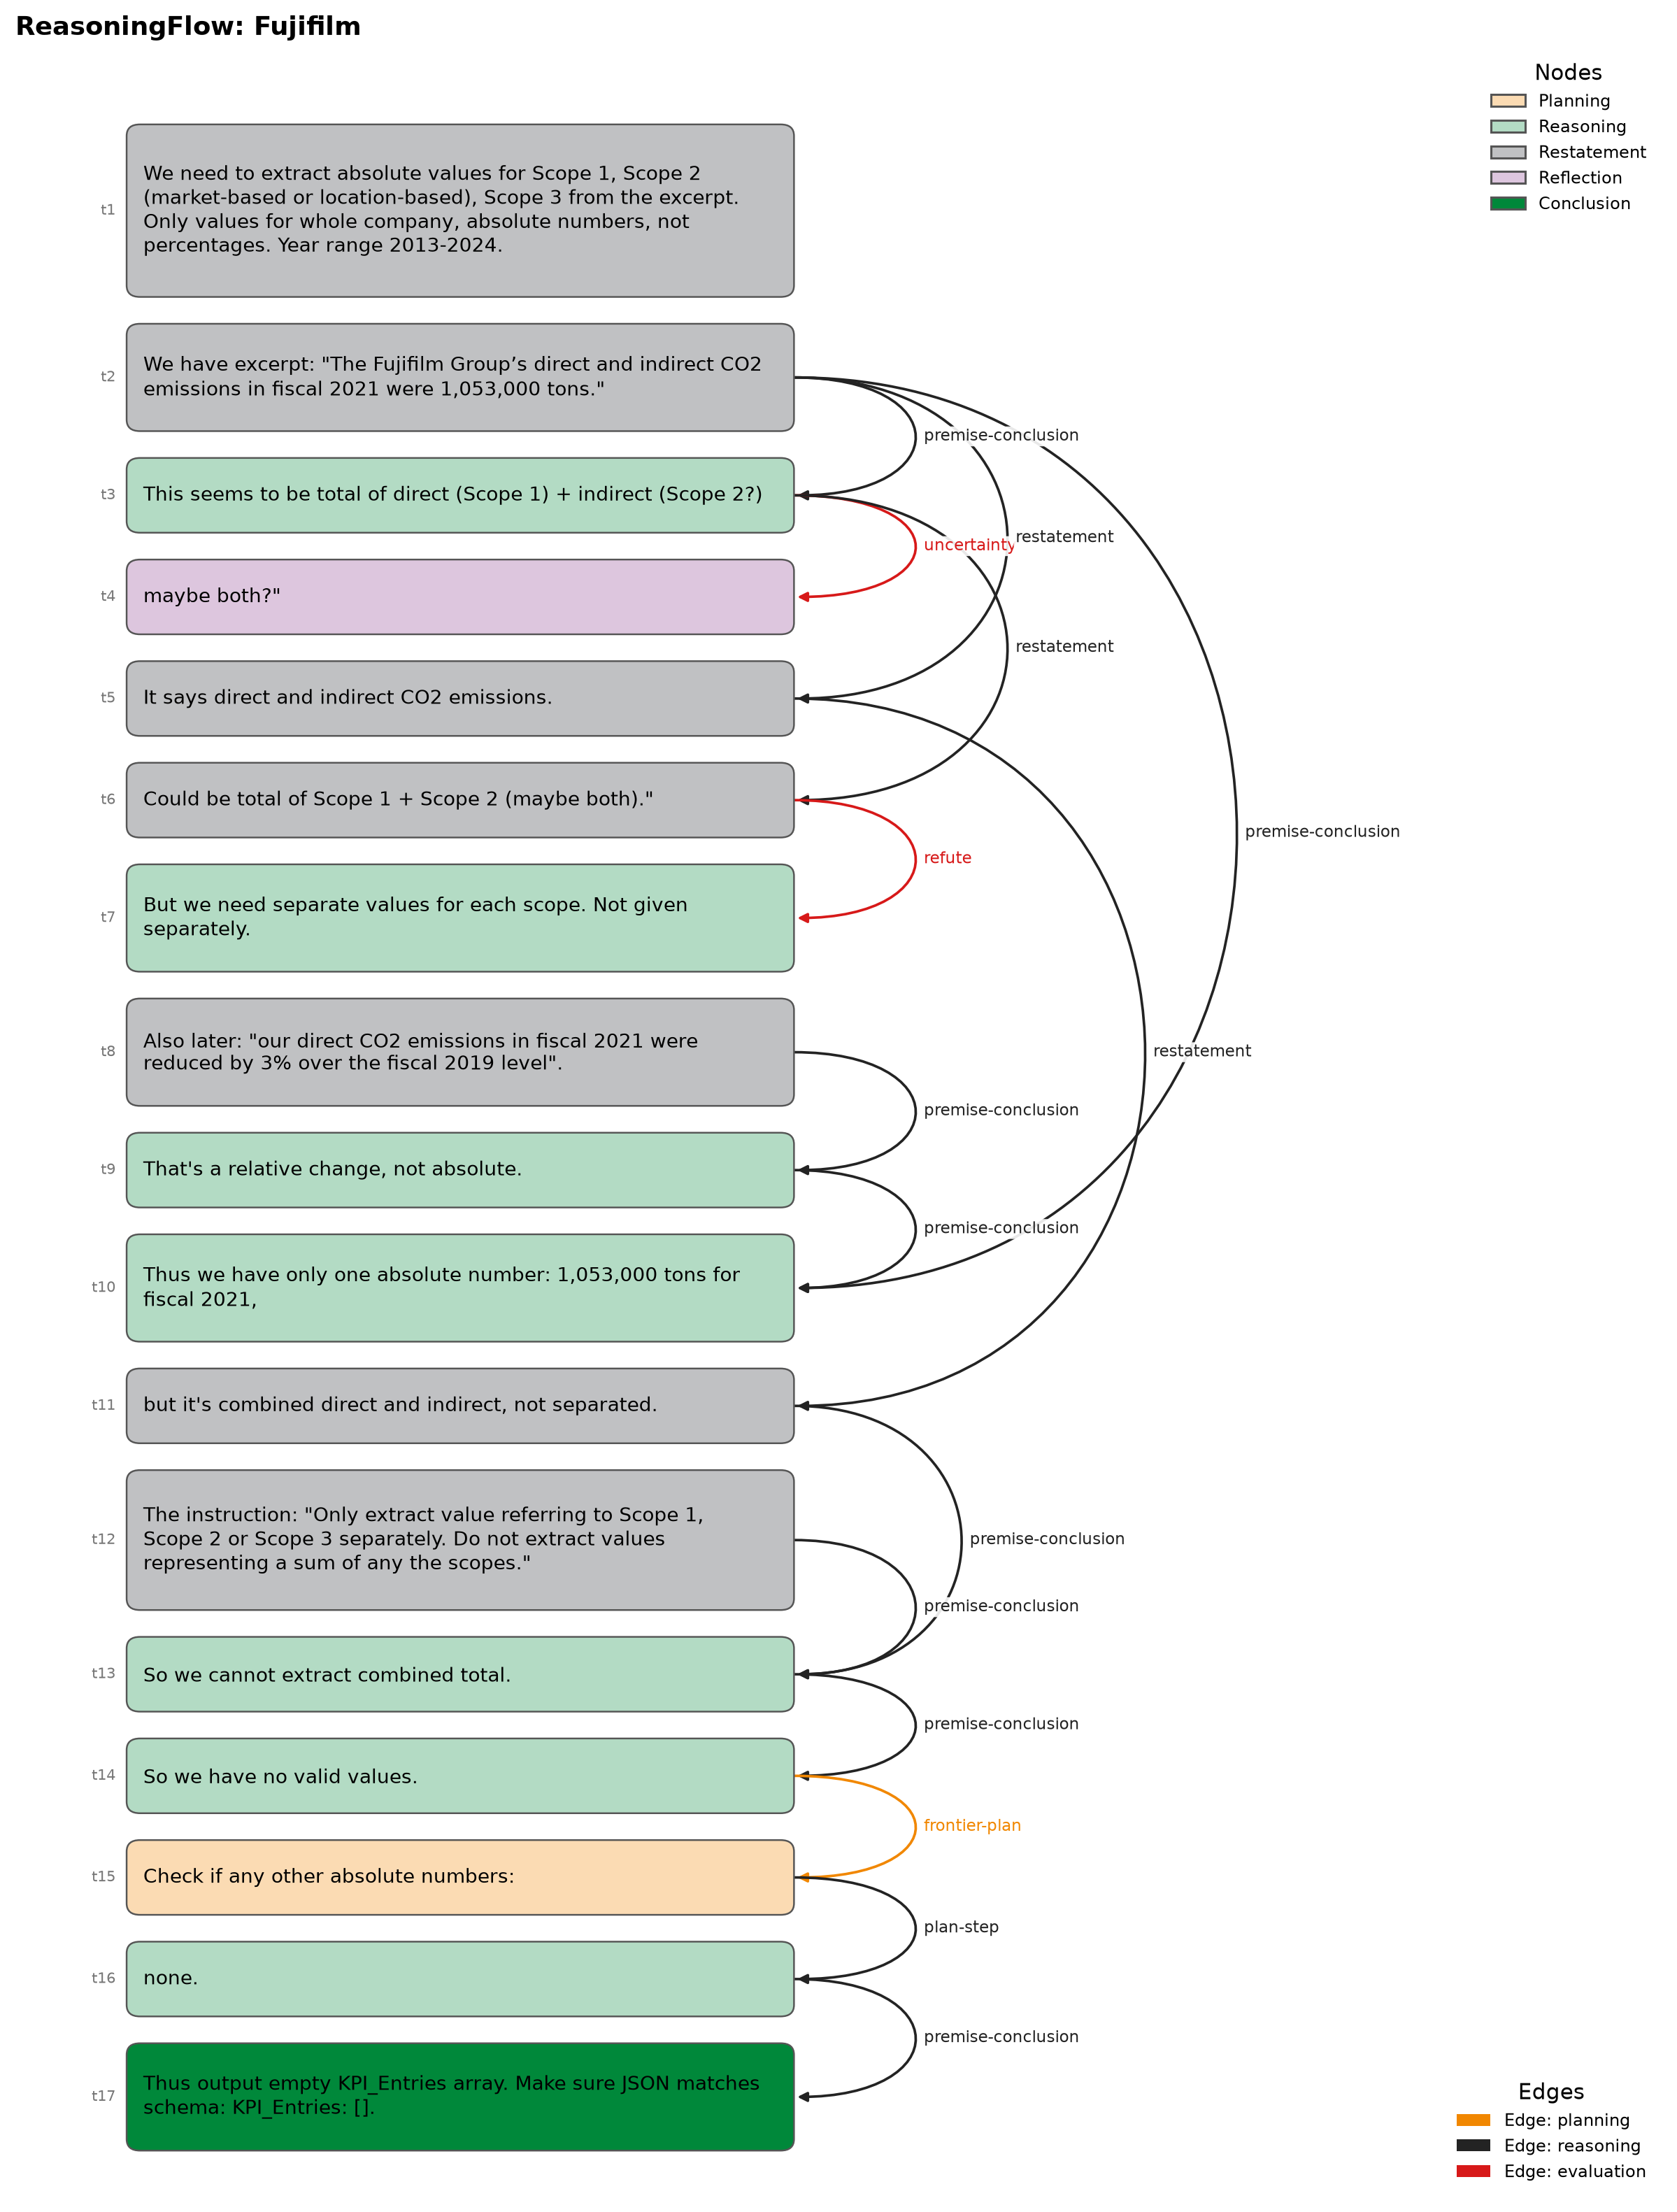
\includegraphics[trim=0pt 0pt 0pt {0.5\imgh}, clip, width=\columnwidth]{presentation/figures/reasoningflow_fujifilm.png}
\end{column}

\end{columns}
\vspace{0.6em}
\centering
{\scriptsize Example trace (gpt-oss, medium) annotated with ReasoningFlow}
\end{frame}

\begin{frame}{ReasoningFlow -- Limitations}
    \begin{itemize}
        \item takes long to annotate one trace manually $\rightarrow$ annotating 4858 traces takes too long
        \item using LLM to annotate $\rightarrow$ risk of mistakes
        \item segment boundaries and categories not always clear
    \end{itemize}
    
\end{frame}

\begin{frame}{3.\ LLM-as-a-Judge}
\begin{itemize}
  \item Idea: let an LLM assign each sentence / span / trace to a category
  \item Useful once a category scheme exists
  \item Can scale beyond manual coding
\end{itemize}
\vspace{0.5em}
\begin{alertblock}{Open point}
Classification is only as good as the category scheme and the prompt / validation setup.
\end{alertblock}
\end{frame}

\begin{frame}{4.\ Error Analysis of Incorrect Traces}
\centering
\renewcommand{\arraystretch}{1.25}
\small
\begin{tabular}{l rr!{\color{lmudark}\vrule width 1.2pt}r}
\toprule
\rowcolor{lmugreen}
\hcell{Model} & \hcell{FP} & \hcell{FN} & \hcell{Total}\\
\midrule
Luna none      & 160 & 48 & 208 \\
\rowcolor{lmulight!60}
GPT-OSS low    & 126 & 123 & 249  \\
GPT-OSS medium & 133 &  77 & 210\\
\rowcolor{lmulight!60}
GPT-OSS high   & 166 &  88 & 254 \\
DeepSeek none  & 179 &  44 & 223 \\
\rowcolor{lmulight!60}
DeepSeek high  &  86 &  71 & 157  \\
DeepSeek max   &  92 &  80 & 172\\
\bottomrule
\end{tabular}

\vspace{0.6em}
{\footnotesize FP: extracted value does not match gold. FN: no extracted value}

\end{frame}

\begin{frame}{5. \ Further Literature}
\begin{itemize}
    \item \textbf{Factuality}
    \item \textbf{Validity}
    \item \textbf{Utility}
    \item \textbf{Coherence}
\end{itemize}
    
\end{frame}

\begin{frame}{Discussion prompts}
\begin{enumerate}
  \item Are Factuality / Validity / Coherence / Utility the right axes for
        \textbf{extraction traces}?
  \item Do we need IE-specific criteria (e.g.\ grounding in the retrieved page)?
  \item Topic modelling first, then map clusters to criteria -- or criteria first,
        then LLM coding?
  \item Sentence-level, span-level, or whole-trace judgements?
\end{enumerate}
\end{frame}

%========================================================================================
\section{Outlook}

\begin{frame}{Outlook}
\begin{itemize}
  \item Agree on a category scheme (literature criteria vs.\ adaptation)
  \item Decide the workflow: topic modelling $\leftrightarrow$ LLM coding
  \item Pilot on a small sample (correct + incorrect pages)
  \item Then relate categories to effort and extraction outcomes -- carefully
\end{itemize}
\end{frame}

{
\usebackgroundtemplate{
\includegraphics[width=\paperwidth]{lmu-background.pdf}}
\setbeamertemplate{headline}{}
\setbeamertemplate{footline}{}
\begin{frame}[plain, noframenumbering]
	\vspace*{3cm}
	{\color{white}\fontsize{28}{32}\selectfont\bfseries Thank you\par}
	\vspace{0.25cm}
	{\color{white}\rule{1.6cm}{1.5pt}\par}
	\vspace{0.35cm}
	{\color{white}\large Discussion\par}
\end{frame}
}

\end{document}
